% Chapter 1

\chapter{Introduction} % Main chapter title

\label{Chapter1} % For referencing the chapter elsewhere, use \ref{Chapter1} 

%----------------------------------------------------------------------------------------
%1 page: Why you do this topic? Relevancy. What's the problem?
%1-2 page(s): What are you doing?
%1 page: Hence, this thesis tries to answer the following research question(s):
%total 4
%----------------------------------------------------------------------------------------

% Define some commands to keep the formatting separated from the content 
\newcommand{\keyword}[1]{\textbf{#1}}
\newcommand{\tabhead}[1]{\textbf{#1}}
\newcommand{\code}[1]{\texttt{#1}}
\newcommand{\file}[1]{\texttt{\bfseries#1}}
\newcommand{\option}[1]{\texttt{\itshape#1}}

%----------------------------------------------------------------------------------------


%1 page: Why you do this topic? Relevancy. What's the problem?
%----------------------------------------------------------------------------------------

Scene understanding is long existing and an interesting area for computer vision. This is highly depended on human visual three dimensional (3D) perception. Understanding the structural dependencies is one of the important task for 3D scene understanding and for its reconstruction, which is basically recovering the range and orientation of the surface and object to mimic the humans visual behaviour \cite{barnard1982computational}. This creates a multiple opportunities for various multimedia computing applications. Most of the time the oblique projection of 3D data into two dimensional(2D) plan is enough for many of our application like 3D displays, movies, games or structural building represtation. But in contrast applications for immersive augmented and virtual reality entertainment, tracking people or objects and observing their activities for robotics or automation for various inductrial and autonomous driving systems etc., having a third dimension data which is depth could be vital. This shows the importance of having 3D depth information for these area of applications. \\

As a solution there are many techniques used to derive depth information which can be categorized into 3. First, dual camera method \cite{li2009dual} second,  dual pixel method \cite{martinello2015dual, choi2017all} and  third sensors based methods \cite{salvi2004pattern}. In extension various methods of estimating depth from focus \cite{grossmann1987depth}, stereo vision \cite{bulthoff1988integration}, and depth from motion \cite{ullman1979interpretation} where also applied. we will discuss more in detail in section \ref{Chapter3:RelatedWork_EarlyApproach}. In this study we are more interested in sensor based methods and there are already some affordable sensing based-technologies for different application were developed. These types of sensors are called structural-light-based (SLB) sensors \cite{salvi2004pattern}, which is based on the projection of structured light \cite{zhang2012microsoft}. Some of the examples for SLB depth sensors are Kinet by Microsoft, Structure Sensor by Occipital, BlasterX Senz3D by Intel Realsense, Leap Motion Sensors by Leap Motion \cite{marin2014hand} and more are available \cite{mal2018sparse}. These devices have proven to have great impact in these areas but its comes with a trade off with ease of use at consumer application end we will discuss more in section \ref{Chapter4:Dataset}. We will be more focused on depth estimation method based on SLB sensors, more specifically Structure Sensor by Occipital in the entire work.\\

Meanwhile as we know there is a remarkable interest grown in brain style computation and Artificial Neural Network (ANNs) is one of its derivative. ANNs have shown great versatility in the field of detection, classification and prediction. ANNs are used for many applications ranging from image processing \cite{guyon1991applications} , audio signal analysis \cite{bourlard1993continuous}, medical \cite{baxt1990use}, business science \cite{widrow1994neural}, music \cite{nadar2019towards} and many more \cite{zhang2000neural}. It  need a careful processing and considerable domain knowledge for representing a raw data into acceptable form for feature learning process. Another import aspect is which comes with brain style computation is hardware limitations towards computational complexity. But in recent days there are significant improvement in the heterogeneous computation \cite{mittal2015survey}. This also comes with difficulties to cope up with low cost and low power platforms for ANNs \cite{mittal2019survey}. \\




\section{Motivation}
\begin{figure}[!b]
    \centering
    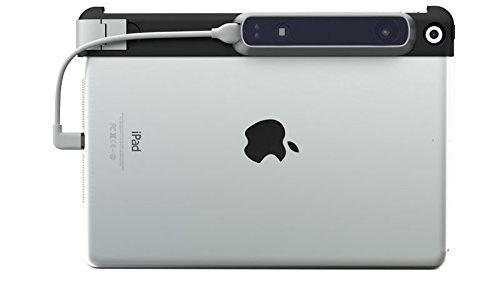
\includegraphics[width = 12cm]{Figures/ipad.jpg}
    \caption{Structural SensorImage Scource: Amazon.com}
    \label{fig:Structural_Sensor}
\end{figure}{}

Having a rich scene understanding of indoor spaces can answer various problems related to robotics, human activity recognition etc. Also in some of the immersive experience and interactive technologies like  virtual reality and augmented reality applications where positional tracking and scene knowledge is crucial element of it.

One of our interest is to achieve full reconstruction of indoor environment. This might lead to various multimedia applications like augmented reality games or productive mobile device applications like \textit{IKEA Place} an application developed by Apple in partnership with Ikea. \textit{IKEA Place} helps you to measure and place a 3D model of furniture from the Ikea catalog \cite{lehnert2017neue}. The furniture represents the app as a 3D model in the appropriate scale. You can walk around the piece of furniture with the camera in hand and look at it from all sides. So the applications of 3D reconstruction of indoor environment can have a wide range of usability. As these applications which we are concerned similar to the one which we just described, are more consumer oriented. Therefore we also want to focus at the consumer level usability of such technology in various fields. This is because even though various efficient methods has been proposed based on the projection of structured light (as discussed in introduction and will be discussed in section \ref{Chapter3:RelatedWork} in detail) are available, the application at the consumer level might be challenging with respect to configuration, portability and background knowledge for usability. As we are discussing at consumer level usability, one of the areas we can look into is portable mobile device cameras. As vast majority of cameras which are shipped today are embedded in mobile devices. These cameras have constraints on physical size, mechanical parts and processing capacity and several solutions have been proposed to measure depth. Photographs from portable mobile devices are found to be a new approach for 3D reconstruction besides various traditional sensor based methods \cite{micheletti2015investigating, adan20113d} in other words 3D image reconstruction from 2D images is our focus and motivation to find a solution in this area. To explain better about the consumer level usability as an example we consider the Structure Sensor manufactured by company called Occipital which is as SLB sensor for portable mobile devides like Apple IPads as show in figure \ref{fig:Structural_Sensor}. This comes with an additional hardware installation. Also there have been some efforts made towards low cost and efficient indoor 3D reconstruction using images collected with portable mobile devices or consumer level cameras \cite{ding2019low} but often time these accuracy or quality of these methods always have a trade off with resources like hardware (using SLB sensors, camera quality) or computational efficiency.

\textit{In summary}, as we understand the importance of depth estimation and its possibilities of remarkable applications in various areas, our motivation in this work is 3D reconstruction of a scene from a given 2D RGB image information which will lead to made consumer level application. For this we also want to answer if we can use brain style computational Artificial Neural Network (ANN) methods. because we believe that by implementing a software based method might reduce the complexity at users end but with a trade off of computational power. We are we observe the growth of computational power we believe its not too far to implement a ANNs models in near future. 



\section{Topic Description}
\label{Chapeter1:Topic_Description}
\begin{figure}[h]
    \centering
    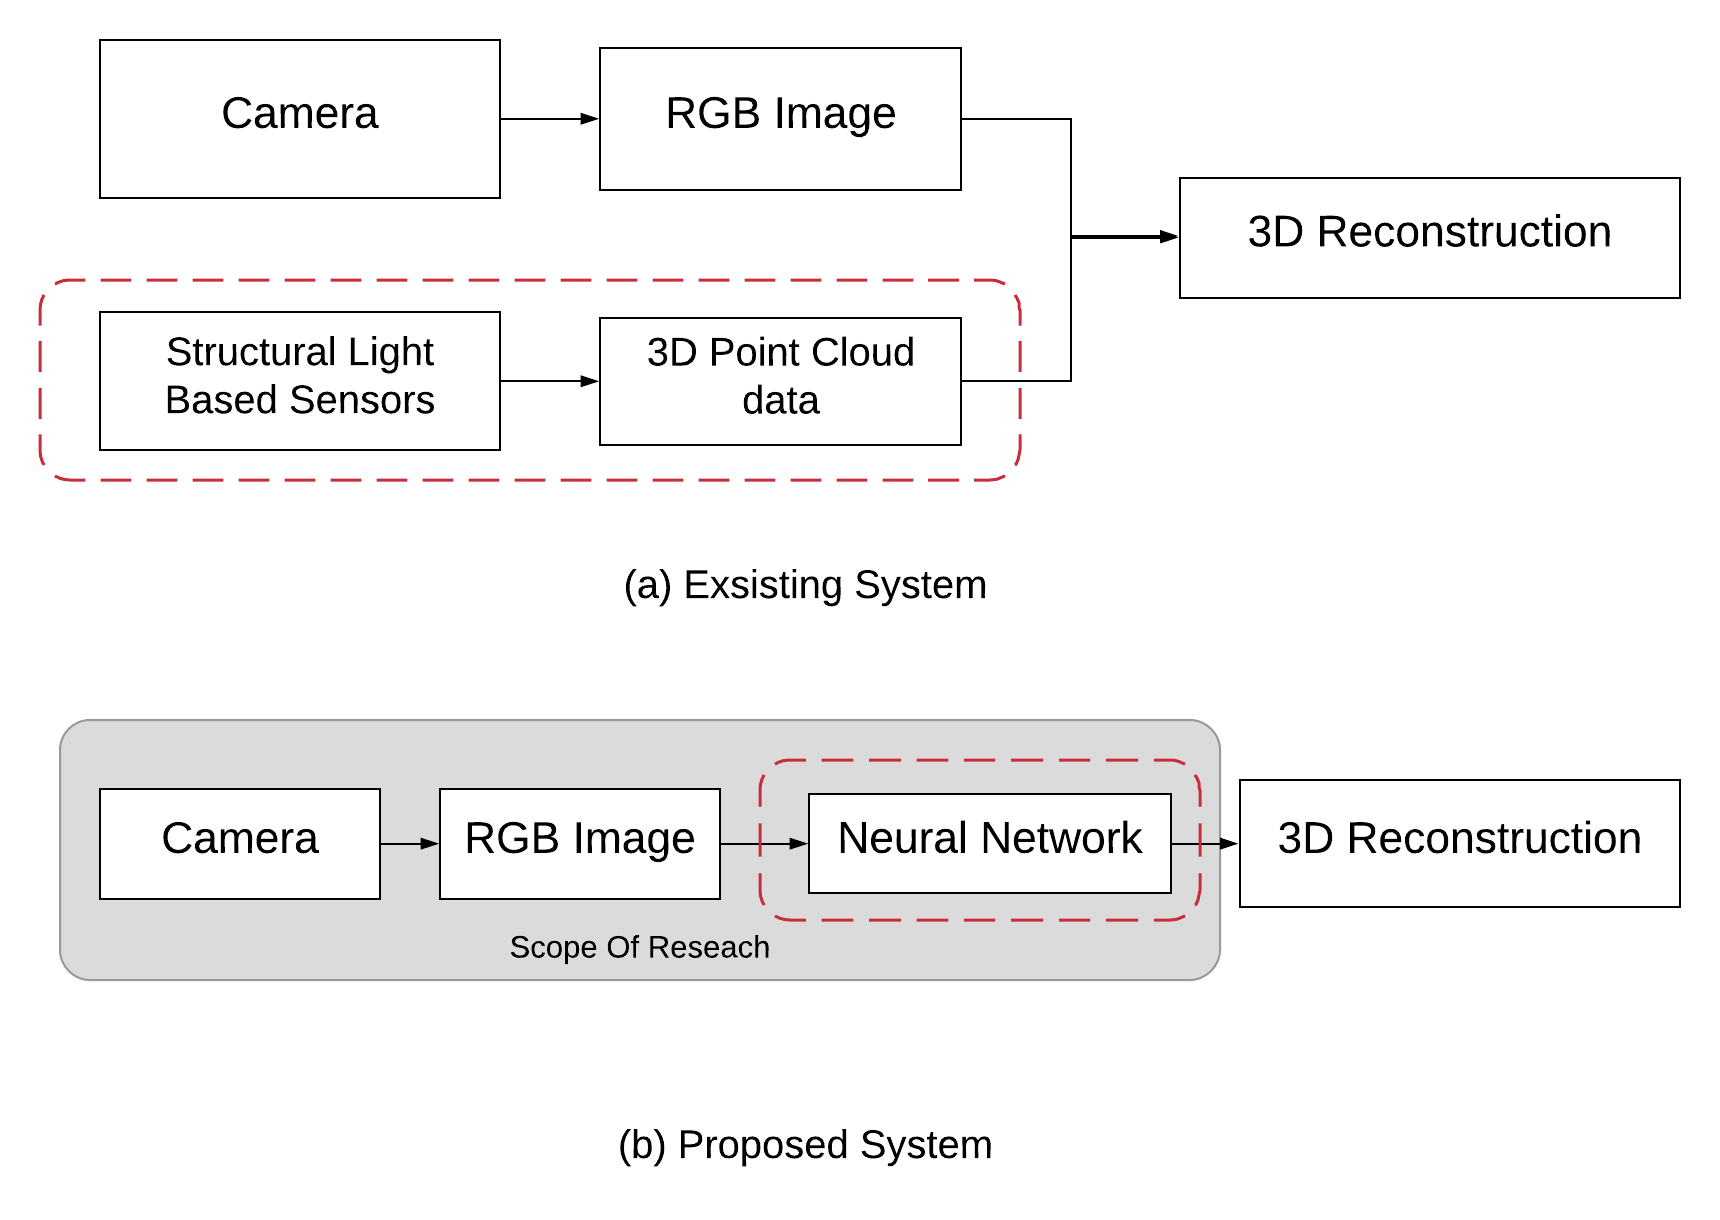
\includegraphics[width = 12cm]{Figures/idea.png}
    \caption{The red box of existing system (a) is replaced by green box proposed method (b)}
    \label{fig:Proposed_Model}
\end{figure}{}
%1-2 page(s): What are you doing?
This study is considering neural networks as an algorithm of depth estimation, more specifically using Convolutions Neural Networks(CNNs). The solution should define concise and accurate pixel for 3D reconstruction. Therefore, the goal is to achieve high accuracy in identifying the depth, especially boundaries of closer objects since the application is in indoor environment. Meanwhile, keeping the network operating speeds at a satisfying level, but the final implementation of this network will be on larger processing unit not in mobile device. This could be achieved by choosing a network architecture wisely with an attention to the details of the problem. Monocular depth estimation is based on ex-ploiting both local properties of texture, gradients, and color, as well as global geometric relations, like relative object placement, and perspective cues \cite{saxena2006learning}. Hence having a global structural understanding of image by Neural Network is very important and at the same time pixel level details for smaller object in a scene. Often time the indoor environment could be more complex than outdoor because of several smaller objects in a scene. For example in office environment, there could be various physical objects on the table where as in outdoor environment having to deal with relatively larger object dimensions are more common.  

Aim of this project is to deliver a robust method and a architecture for depth image prediction replacing the sensor. As shown in figure \ref{fig:Proposed_Model} (a) Existing System for 3D reconstruction relay on hardware based implementation of a SLB sensor which is Structure Sensor figure \ref{fig:Structural_Sensor} integrated with IPad. This is done using Apple AR kit implementation which gives 2D RGB image from IPad and its depth information from the Structure sensor and together are send for further processing of 3D reconstruction. First our primary goal is to replace the existing system highlighted in red box in figure \ref{fig:Proposed_Model} (a) Existing System with a Neural Network as shown in highlighted box in \ref{fig:Proposed_Model}(b) Proposed System. We take advantage of Neural network as this has proven to give great results which we will see in details in section \ref{Chapter3:RelatedWork}.


Secondly, existing solutions to depth estimation from a single image usually rely on assumptions all the far field depth are mapped to a certain threshold which can result as a wall in 3D reconstruction from 2D. For example, the depth range of Kinet v2 sensor range from 0.5 meters (m) to 4.5m, most of work to our knowledge are based on neural network the range above 4.5m are mapped to the maximum value 4.5m \cite{Silberman:ECCV12} which results as a wall. In practical implementation for 3D reconstruction its undesirable for us to have wall. Whereas the output from SLB or Kinet sensors gives a dead pixel (no pixel) or holes for range above any threshold (for Kinet v2 is 4.5m). Another very important reason for having dead pixel is to get perfect reconstruction - ideally we can repaint the dead pixel by changing the position of camera, hence rather than approximation the values around dead pixel and removing dead pixel its important for us to have information about these dead pixel. In our work we are also interested to address this problem. We wanted the the network to learn these dead pixels as true SLB sensors along with the relative depth of the scene for efficient regeneration of 3D scene. 

These two problems gives us a clear direction to formulates some of the specific questions to be answered in this work which is described below. 


\section{Research question(s) and scientific contribution(s)}
%1 page: Hence, this thesis tries to answer the following research question(s):

This work tries to address the following two questions:
\begin{itemize}
    \item RQ1: Can we Neural Network work as good as SLB sensor in predicting relative depth of a scene?
    \item RQ2: Can a network learn to regenerate the dead pixel from a given 2d image?
    \item RQ3: Can Network learn Different Camera intrinsic parameters?  
\end{itemize}

In order to answer the three questions mentioned above, we propose a state-of-the-art approach using neural networks for this problem. Also generation of a new dataset is required to answer RQ2 and RQ3. This is because most of the approach does not focus in retrieving the dead pixels and existing dataset \nadacn{toShivam: Cite NYU, Make3D and relevant indoor dataset} fail to provide with the dead pixel except NYUv2 dataset with contains raw data information we will discuss more about the dataset in detain in section \ref{Chapter4:Dataset}. To give a jutified reson for RQ3, we need to generate new dataset to have a common ground for comparison. 

Our main two contribution for this work are, first Proposed a neural network model for depth map generation. Secondly we generated new dataset based on Structural (SLB) Sensor.


As we understand that our goal for this work is to achieve a similar working neural network model replacing Structural (SLB) sensor. This might reduce the complexity in users with a trade off of computational power. In this initial phase of research our scope of study how to generate the 3D depth maps from neural networks after training on similar depth data, so all the computation are tested with high processing unit \textit{Nvidia Quadro RTX 8000} graphic card with Graphics processor memory 48 GB GDDR6 with ECCRTX-OPS 84T \nadacn{write about power consumption}. 
And knowing that the final implementation of the Neural Network model will on larger processor but not embedded in mobile device, gives a space of implementing larger and efficient network architecture. 
